% Created:  
% Author:   Julie Sewards
% Filename: background.tex

\chapter{Background Material}
\label{cha:background}

In this chapter we will introduce some key aspects of the android architecture and its security features.  We will also examine the features offered by the Dropbox API and finally we will look briefly at some of the commercial applications which were reviewed as part of our initial research and which offer some features similar to Securely Share.

\section{Android Security Features}

Android provides an open source platform and application environment for mobile devices.  It has a layer based architecture whose foundational component  is the Android Operating System.  Based on the tried and tested Linux kernel and modified by Google to include some additional features, it is the comprehensive user permissions model inherent in Linux that is responsible for providing the separation between applications that is a key feature of Android security.  At installation time, each application is assigned a unique user ID (UID);at runtime each application is run as a separate process an as a separate user with its given UID. This creates an Application Sandbox, protecting any resources belonging to that application (memory space, files, etc.) from being accessed by another application unless specifically permitted to do so by the developer.

\begin{figure}[h!]
    \centering
    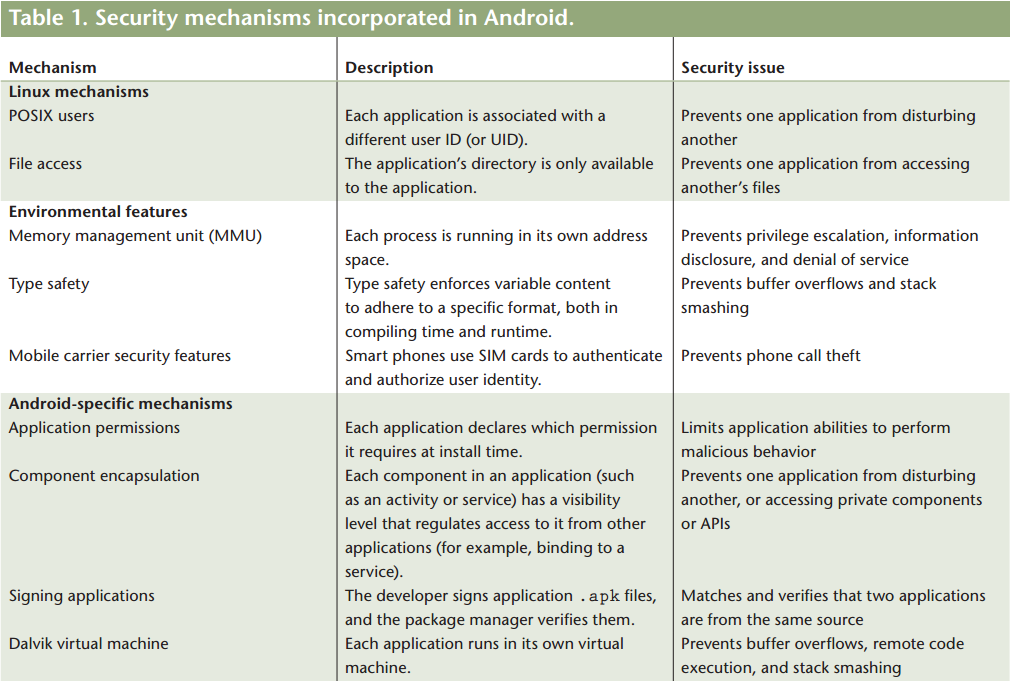
\includegraphics[width=0.99\textwidth]{security_table}                                                                                                                                                                                                                                                                                                                                                                                                                                                                                                                                                                                                                                                                                                                                                                                                                                                                                                                                                                                                                                                                                                                                                                                                                                                                                                                                                                                                                                                                                                                                                                                                                                                                                                                                                                                                                                                                                                                                                                                                                                                                                                                                                                                                                                                                                                                                                                                                                                                                                                                                                                                                                                                                                                                                                                                                                                                                                                                                                                          
\caption[Security table]{Security mechanisms incorporated in Android \citep{shabtai2010google}}\label{fg:overview_pyramid}
        \label{fig:table}
\end{figure}

Android also provides some additional security mechanisms. Most relevant to our application is the requirement that each application requiring certain restricted permissions (write to external storage, access network, access contacts, etc.) has to declare them and the user is alerted and asked to confirm this access at installation time.  Figure \ref{fig:table} provides a useful summary of these mechanisms and the related security issues.

\subsubsection*{KeyStore}

Another of Android's security mechanisms is the KeyStore which is designed for securing cryptographic artefacts.  Although frequently associated with the process of digitally signing applications for release, they can more generally be used for storing certificates, private keys, and even symmetric keys.  Each KeyStore is secured using Password Based Encryption (PBE) with a user supplied password and may also use separate passwords for each individual entry.



\section{Dropbox API}
\label{sec:dropbox}
Dropbox is a cloud storage service that also offers users  automatic backup facilities, file synchronization across devices, and the ability to share files with other users.  It provides multi-platform client applications plus a series of public APIs that enable different subsets of the Dropbox functionality to be integrated into third-party applications.  

On the Android platform, Dropbox offers three APIs, described on its website as follows:-
\begin{description}
	\item[Core]The Core API includes the most comprehensive functionality including features such as search, file restore, etc. Although more complex than either of the other two to implement, it is often more suitable when developing server-based apps.
	\item[Datastore]The Datastore API provides a means of storing and synchronizing structured data like contacts, to-do items, and game states across  all the user's devices.
	\item[Sync]The Sync API provides a file system for accessing and writing files to the user's Dropbox.  The Sync API manages the process of synchronizing file changes to Dropbox and can also provide the app with notification when changes are made to files stored on the server.
\end{description}

For the purposes of the SecurelyShare app, although it offers the most basic interface to the Dropbox server, the Sync API was deemed to support both the functionality required for the prototype and some additional facilities which could be implemented at a later date in order to improve the overall user experience.

Each app on the Dropbox Platform needs to be registered in the App Console and the developer needs to select which permissions the app requires. These permissions determine the type of data that the app can access in the user's Dropbox.  For the Sync API, three levels of permission were available:
\begin{enumerate}
\item App folder:  this creates a folder in the user's Dropbox with the same name as the app, all files relating to the app are kept here and access is restricted to this folder and its subfolders.
\item File type: the app is given access to the user's entire Dropbox but is restricted only to seeing files of certain types (documents, images, ebooks, etc.)  
\item Full Dropbox:  the app is given unrestricted access to the user's Dropbox
\end{enumerate}
Developers are also able to submit a request to use a custom file extension with the File type permission.


\section{Review of Related Work }
\label{sec:agke}
\red{ was intending to include a summary of all the material relating to key distribution that I reviewed - not sure if I am going to be able to do this now }\\

\section{Review of Other Products}
\label{sec:other}
One of the security claims of cloud storage provider, Dropbox, is that user data stored on their servers is  fragmented and encrypted using 256-bit AES.  However, although users may feel reassured by these claims, it is also to be noted that since this encryption is applied server-side, the servers also have access to the keys required to decrypt this information.  Furthermore, the   Dropbox privacy policy states that,  
\begin{quotation}
"We may disclose your information to third parties if we determine that such disclosure is reasonably necessary to (a) comply with the law; (b) protect any person from death or serious bodily injury; (c) prevent fraud or abuse of Dropbox or our users; or (d) protect Dropbox's property rights." 
\end{quotation} 

It may therefore come as little surprise that there are an increasing  number of client-side encryption applications available that  integrate with Dropbox and other similar cloud services  to ensure that, even if files are disclosed, the service providers would have no access to decryption keys.
Although there are a significant number of encryption applications available for Android, most were discarded for consideration here as they are primarily designed for a single user to encrypt files prior to cloud storage and had little or no support for key sharing.  

When trying to evaluate these products there appeared to be a marked absence of robust reviews from respected members of the security fraternity; many of the review that were available seemed to focus more on the usability of applications rather than on their security features.  We chose three commercially produced applications to consider in greater depth, Boxcryptor, Viivo and SafeMonk.  These were selected partly because they seemed to attract most mentions (although that may simply be due to the fact that they were commercial products and hence had larger marketing budgets), but also because we were able to find some level of technical description of the security protocols used.  There was a common trend among the examined applications to use AES for encryption of user files and some implementation of RSA to manage the key exchange, All three applications used a central server  for key management, although each was keen to stress that they had no access to key material that would enable them to decrypt user files. 

Boxcryptor and Safemonk both store the user's private key on the server, their justification being that it would allow the user to install the application on multiple devices and they both used password-based encryption (PBE) in order to secure the key on the server.  Although the servers use key-stretching algorithms to derive the encryption keys, we should always be aware that users can be very poor at choosing strong passwords and at keeping them secure. (In a study of password reuse, Bonneau \cite{das2014tangled} observed that 43 percent of  users reused a password across multiple sites)




